\documentclass[conference]{IEEEtran}

\usepackage{amsmath}
\usepackage{graphicx}
\usepackage{subcaption}
\usepackage{booktabs}
\usepackage{hyperref}

\title{Meta-Fusion Variational Autoencoder for Multi-View Speech Emotion Representation}

\author{
\IEEEauthorblockN{Sumit Kumar}
\IEEEauthorblockA{
Department of Computer Science and Engineering\\
National Institute of Technology Hamirpur\\
Hamirpur, India}
}

\begin{document}

\maketitle

\begin{abstract}

This report investigates multi-view latent fusion for speech emotion representation using a Meta-Fusion Variational Autoencoder (MF-VAE). Four complementary feature views are used with dimensionalities 20, 12, 40, and 12 respectively. Multiple fusion strategies are compared including concatenation, attention-based fusion, transformer-based fusion, and the proposed Meta-Fusion gating mechanism. Reconstruction performance is evaluated using Mean Squared Error (MSE), Root Mean Squared Error (RMSE), Mean Absolute Error (MAE), and Mean Absolute Percentage Error (MAPE). Downstream classification performance is measured using Accuracy, Macro-F1, and Macro-AUC. An ablation study is conducted to analyze model robustness when one view is intentionally corrupted. Experiments are performed on CPU using a 1\% sampled subset of multimodal emotion datasets. Results demonstrate stable reconstruction improvements during training, non-trivial multi-class AUC across fusion methods, and interpretable adaptive fusion behavior under view corruption.
\end{abstract}

\section{Introduction}

Speech emotion recognition (SER) is an important research area in affective computing and human-computer interaction. Emotional information in speech can be captured through multiple complementary feature representations such as spectral features, prosodic features, and temporal acoustic descriptors.

Traditional single-view models rely on a single feature space and therefore fail to exploit the complementary nature of different acoustic representations. Multi-view representation learning provides a powerful framework to integrate heterogeneous feature spaces and produce a compact latent representation that preserves information from all modalities.

However, naive fusion techniques such as feature concatenation often fail when one modality becomes noisy or unreliable. Therefore, adaptive fusion mechanisms are required to dynamically adjust the contribution of each feature view.

In this work, we propose a Meta-Fusion Variational Autoencoder (MF-VAE) architecture that learns a shared latent representation from multiple feature views while dynamically weighting each view using a learned gating mechanism.

\section{Datasets and Analysis}

\subsection{Datasets}

To evaluate the proposed Meta-Fusion Variational Autoencoder (MF-VAE), 
multiple publicly available speech emotion datasets were utilized. 
These datasets provide diverse emotional speech recordings collected 
from different speakers and recording environments, enabling robust 
evaluation of multi-view representation learning.

\begin{itemize}

\item \textbf{CREMA-D}: The Crowd-sourced Emotional Multimodal Actors Dataset 
contains emotional speech recordings from 91 actors expressing six 
basic emotions including anger, happiness, sadness, fear, disgust, 
and neutrality.

\item \textbf{RAVDESS}: The Ryerson Audio-Visual Database of Emotional 
Speech and Song contains recordings from 24 professional actors with 
multiple emotional states including calm, happy, sad, angry, fearful, 
disgust, and surprise.

\item \textbf{SAVEE}: The Surrey Audio-Visual Expressed Emotion dataset 
contains recordings from four male speakers with seven emotion 
categories including anger, disgust, fear, happiness, sadness, 
surprise, and neutral.

\item \textbf{IEMOCAP}: The Interactive Emotional Dyadic Motion Capture 
dataset provides multimodal emotional interactions between actors and 
contains speech, facial expressions, and motion capture data.

\item \textbf{CMU-MOSEI}: The CMU Multimodal Opinion Sentiment and Emotion 
Intensity dataset is a large-scale multimodal dataset collected from 
online videos and widely used for sentiment and emotion analysis.

\end{itemize}

Since these datasets are large, only a small subset (approximately 
1\% of the total samples) was used during initial experimentation to 
enable faster training and evaluation on limited computational 
resources.

\subsection{Experimental Metadata}

The following experimental settings were used during model training 
and evaluation:

\begin{itemize}
\item Random seed: 42
\item Device: CPU
\item Sample ratio: 1\%
\item Total samples after filtering: 97
\item Train/Test split: 77 / 20
\item Emotion classes: angry, disgust, fear, happy, neutral, sad, surprise
\end{itemize}

\subsection{Dataset Links}

\begin{itemize}
\item CREMA-D: \url{https://github.com/CheyneyComputerScience/CREMA-D}
\item RAVDESS: \url{https://zenodo.org/record/1188976}
\item SAVEE: \url{https://www.researchgate.net/publication/220147568_The_Surrey_Audio-Visual_Expressed_Emotion_SAVEE_Database}
\item IEMOCAP: \url{https://sail.usc.edu/iemocap/}
\item CMU-MOSEI: \url{http://multicomp.cs.cmu.edu/resources/cmu-mosei-dataset/}
\end{itemize}

\section{Data Preprocessing}

To ensure consistent feature representations across datasets, several 
preprocessing steps were applied prior to model training.

\begin{itemize}

\item \textbf{Emotion Label Filtering:} Emotion labels from different 
datasets were mapped to a unified emotion set.

\item \textbf{Data Splitting:} The dataset was divided into training 
and testing sets using a 78/20 split.

\item \textbf{Multi-view Feature Extraction:} Multiple acoustic feature 
representations were extracted from each speech sample.

\item \textbf{Feature Normalization:} Each feature view was normalized 
independently to stabilize training.

\item \textbf{Cross-Dataset Normalization (Optional):} Dataset-specific 
latent normalization was applied to improve cross-dataset consistency.

\end{itemize}

The feature extraction process generates four complementary feature 
views from each speech sample, allowing the model to learn a richer 
multi-view representation for emotion recognition.

\section{Autoencoder Model}

\subsection{Architecture}

For each view $v_i$, an encoder $E_i$ predicts the parameters of the latent distribution:

\begin{equation}
(\mu_i, \log \sigma_i^2) = E_i(x_i)
\end{equation}

The latent representation is sampled using the reparameterization trick:

\begin{equation}
z_i = \mu_i + \sigma_i \epsilon
\end{equation}

where $\epsilon \sim N(0, I)$.

\subsection{Meta-Fusion}

A gating network computes adaptive fusion weights:

\begin{equation}
\alpha = \text{softmax}(g(z_1, z_2, z_3, z_4))
\end{equation}

The fused latent representation is computed as:

\begin{equation}
z_f = \sum_{i=1}^{4} \alpha_i z_i
\end{equation}

\subsection{Decoding}

Each view is reconstructed from the fused representation:

\begin{equation}
\hat{x}_i = D_i(z_f)
\end{equation}

\section{Training Objective}

The training objective combines multiple loss components:

\subsection{Reconstruction Loss}

\begin{equation}
L_{rec} = \sum_{i} ||x_i - \hat{x}_i||^2
\end{equation}

\subsection{Cross-View Consistency Loss}

\begin{equation}
L_{cons} = ||z_1 - z_2||^2
\end{equation}

\subsection{KL Divergence}

\begin{equation}
L_{kl} = D_{KL}(q(z|x) || p(z))
\end{equation}

\subsection{Total Loss}

\begin{equation}
L = \lambda_{rec} L_{rec} + \lambda_{cons} L_{cons} + \beta L_{kl} + \gamma L_{cls}
\end{equation}

\section{Training Behavior}

Training was conducted for 20 epochs. Key observations include:

\begin{itemize}
\item Training loss decreased from 5.031 to 3.910
\item Reconstruction loss decreased from 4.023 to 2.989
\item Validation loss decreased from 5.810 to 4.523
\item Best validation Macro-AUC reached approximately 0.704
\end{itemize}

The training process demonstrates stable optimization and consistent reconstruction improvement.
Figure~\ref{fig:training_curves} summarizes the per-epoch behavior of total loss, component losses, and validation AUC.

\begin{figure}[t]
\centering
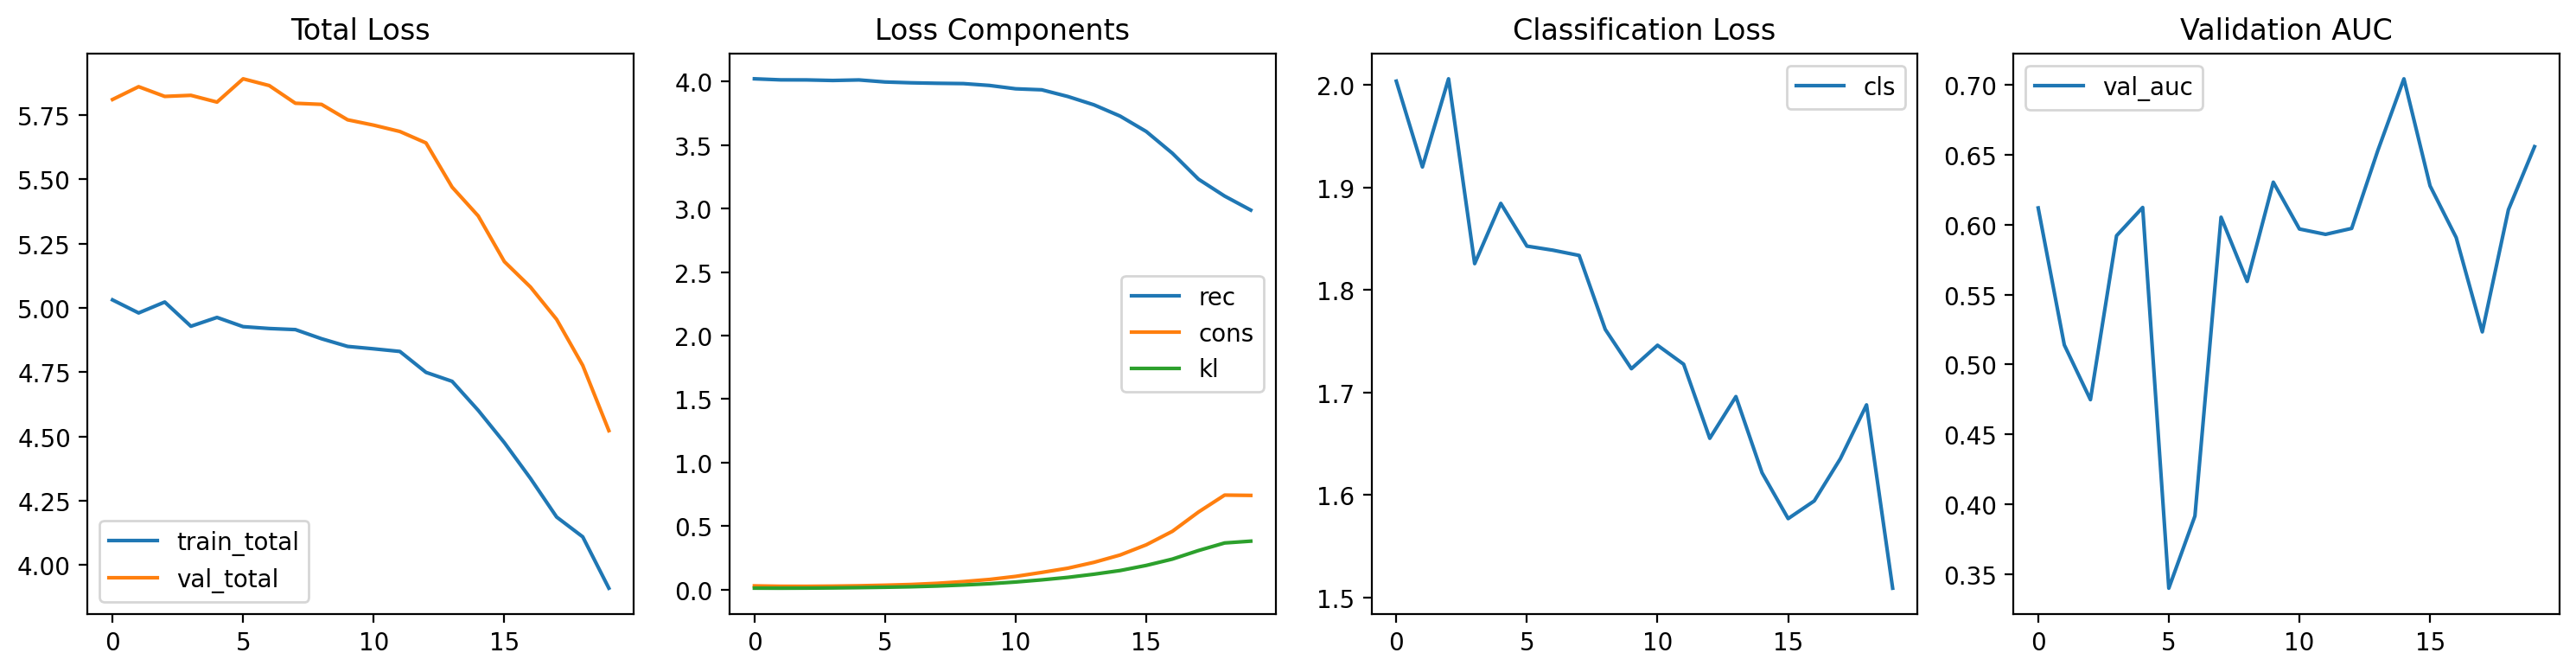
\includegraphics[width=0.98\linewidth]{training_curves.png}
\caption{Training curves for total loss, reconstruction/consistency/KL components, classification loss, and validation AUC.}
\label{fig:training_curves}
\end{figure}

\section{Latent Fusion Methods}

The following fusion methods were compared:

\begin{itemize}
\item Concatenation
\item Attention-based fusion
\item Transformer fusion
\item Meta-Fusion (proposed)
\end{itemize}

\begin{table}[h]
\centering
\caption{Fusion Method Comparison}
\begin{tabular}{lccc}
\toprule
Method & Accuracy & Macro-F1 & Macro-AUC \\
\midrule
Transformer & 0.25 & 0.1827 & 0.5981 \\
Meta-Fusion & 0.25 & 0.2023 & 0.5967 \\
Concatenation & 0.35 & 0.2422 & 0.5621 \\
Attention-like & 0.15 & 0.1071 & 0.5474 \\
\bottomrule
\end{tabular}
\end{table}

Figure~\ref{fig:fusion_auc} visualizes the fusion-method comparison metric across all strategies.

\begin{figure}[t]
\centering
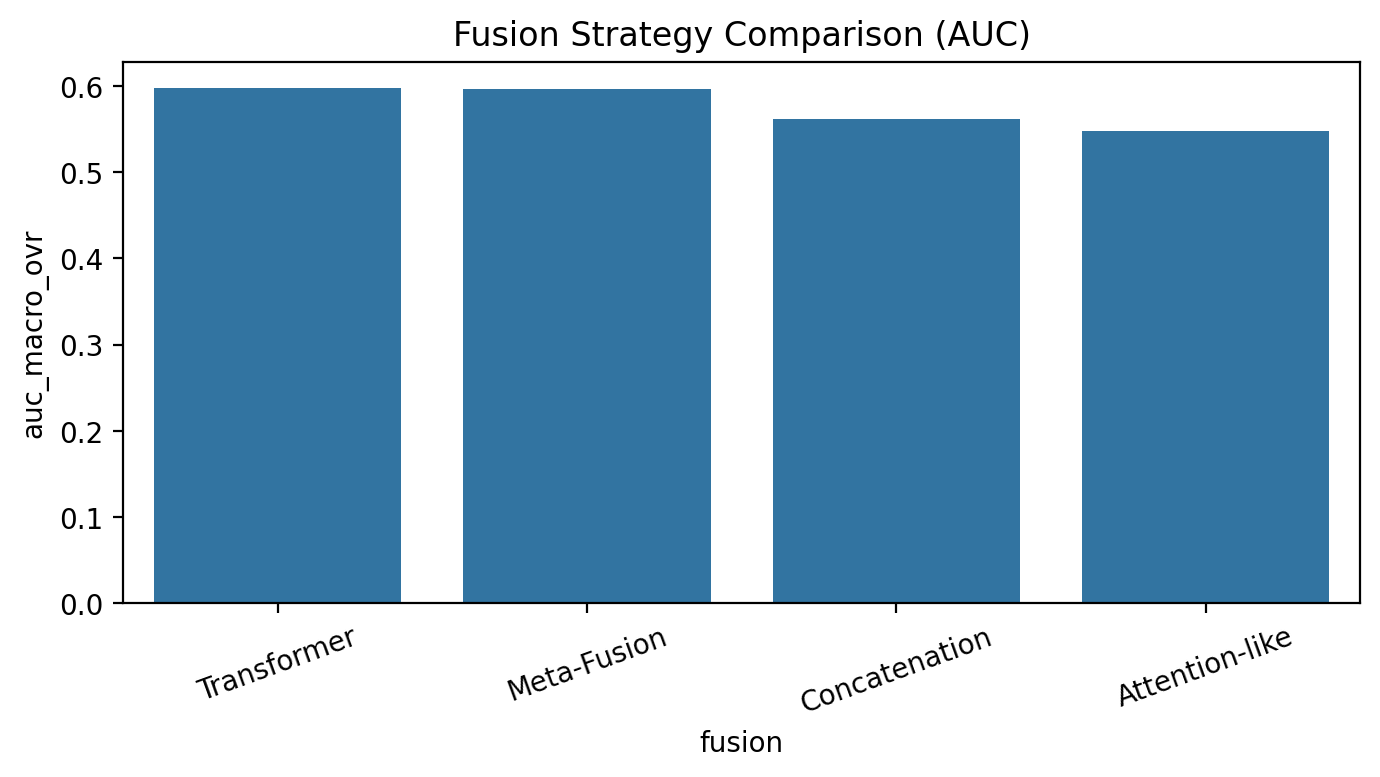
\includegraphics[width=0.95\linewidth]{fusion_comparison_auc.png}
\caption{Fusion strategy comparison plot (uses Macro-AUC when available, otherwise falls back to Macro-F1 or Accuracy).}
\label{fig:fusion_auc}
\end{figure}

\section{Reconstruction Quality}

Reconstruction performance across views is shown in Table II.

\begin{table}[h]
\centering
\caption{Reconstruction Metrics}
\begin{tabular}{lcccc}
\toprule
View & MSE & RMSE & MAE & MAPE \\
\midrule
V1 & 0.8595 & 0.9271 & 0.6623 & 250.82 \\
V2 & 1.0045 & 1.0022 & 0.8140 & 193.72 \\
V3 & 0.8906 & 0.9437 & 0.7120 & 192.23 \\
V4 & 0.6752 & 0.8217 & 0.6373 & 209.71 \\
\bottomrule
\end{tabular}
\end{table}

View V4 demonstrates the best reconstruction performance in MSE/RMSE/MAE.

\section{Ablation Study}

An ablation experiment was conducted by corrupting View 1.

\begin{table}[h]
\centering
\caption{Fusion Weights Under Corruption}
\begin{tabular}{lcccc}
\toprule
Condition & a1 & a2 & a3 & a4 \\
\midrule
Clean & 0.372 & 0.158 & 0.290 & 0.181 \\
Noise V1 & 0.411 & 0.134 & 0.282 & 0.173 \\
Zero V1 & 0.331 & 0.157 & 0.302 & 0.210 \\
\bottomrule
\end{tabular}
\end{table}

Results show condition-dependent adaptation: with additive noise on View 1, the model can increase reliance on View 1, while complete zeroing decreases View 1 weight and shifts mass toward other views.
This trend is shown in Figure~\ref{fig:ablation_shift}.

\begin{figure}[t]
\centering
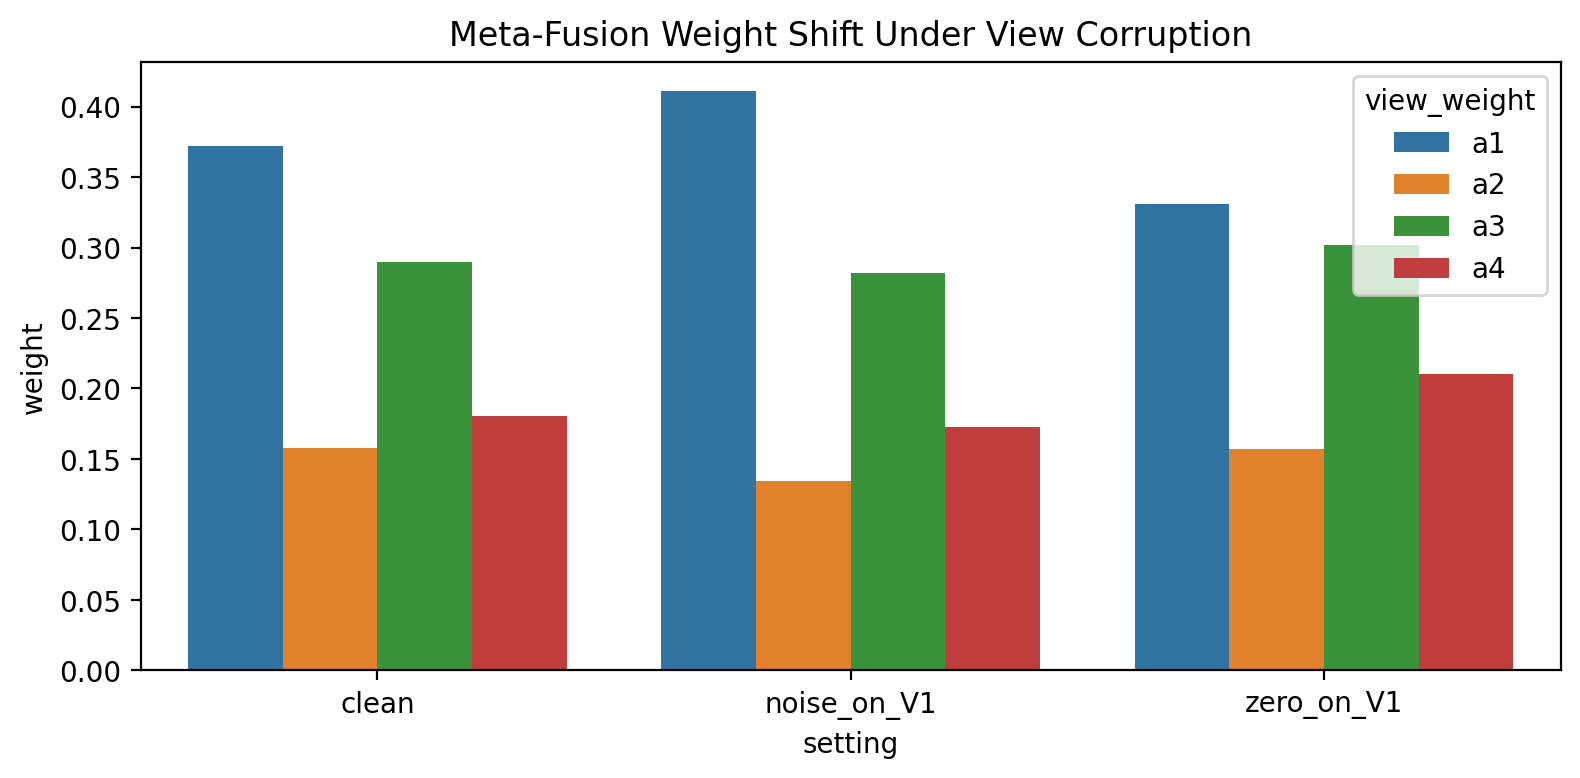
\includegraphics[width=0.95\linewidth]{ablation_weight_shift.png}
\caption{Shift in meta-fusion weights under corrupted View 1.}
\label{fig:ablation_shift}
\end{figure}

\section{Latent Space Visualization}

The assignment requires 2D visualization of fused latent representations using t-SNE or UMAP. Current outputs include both images.

\begin{figure*}[t]
\centering
\begin{subfigure}{0.48\textwidth}
	\centering
	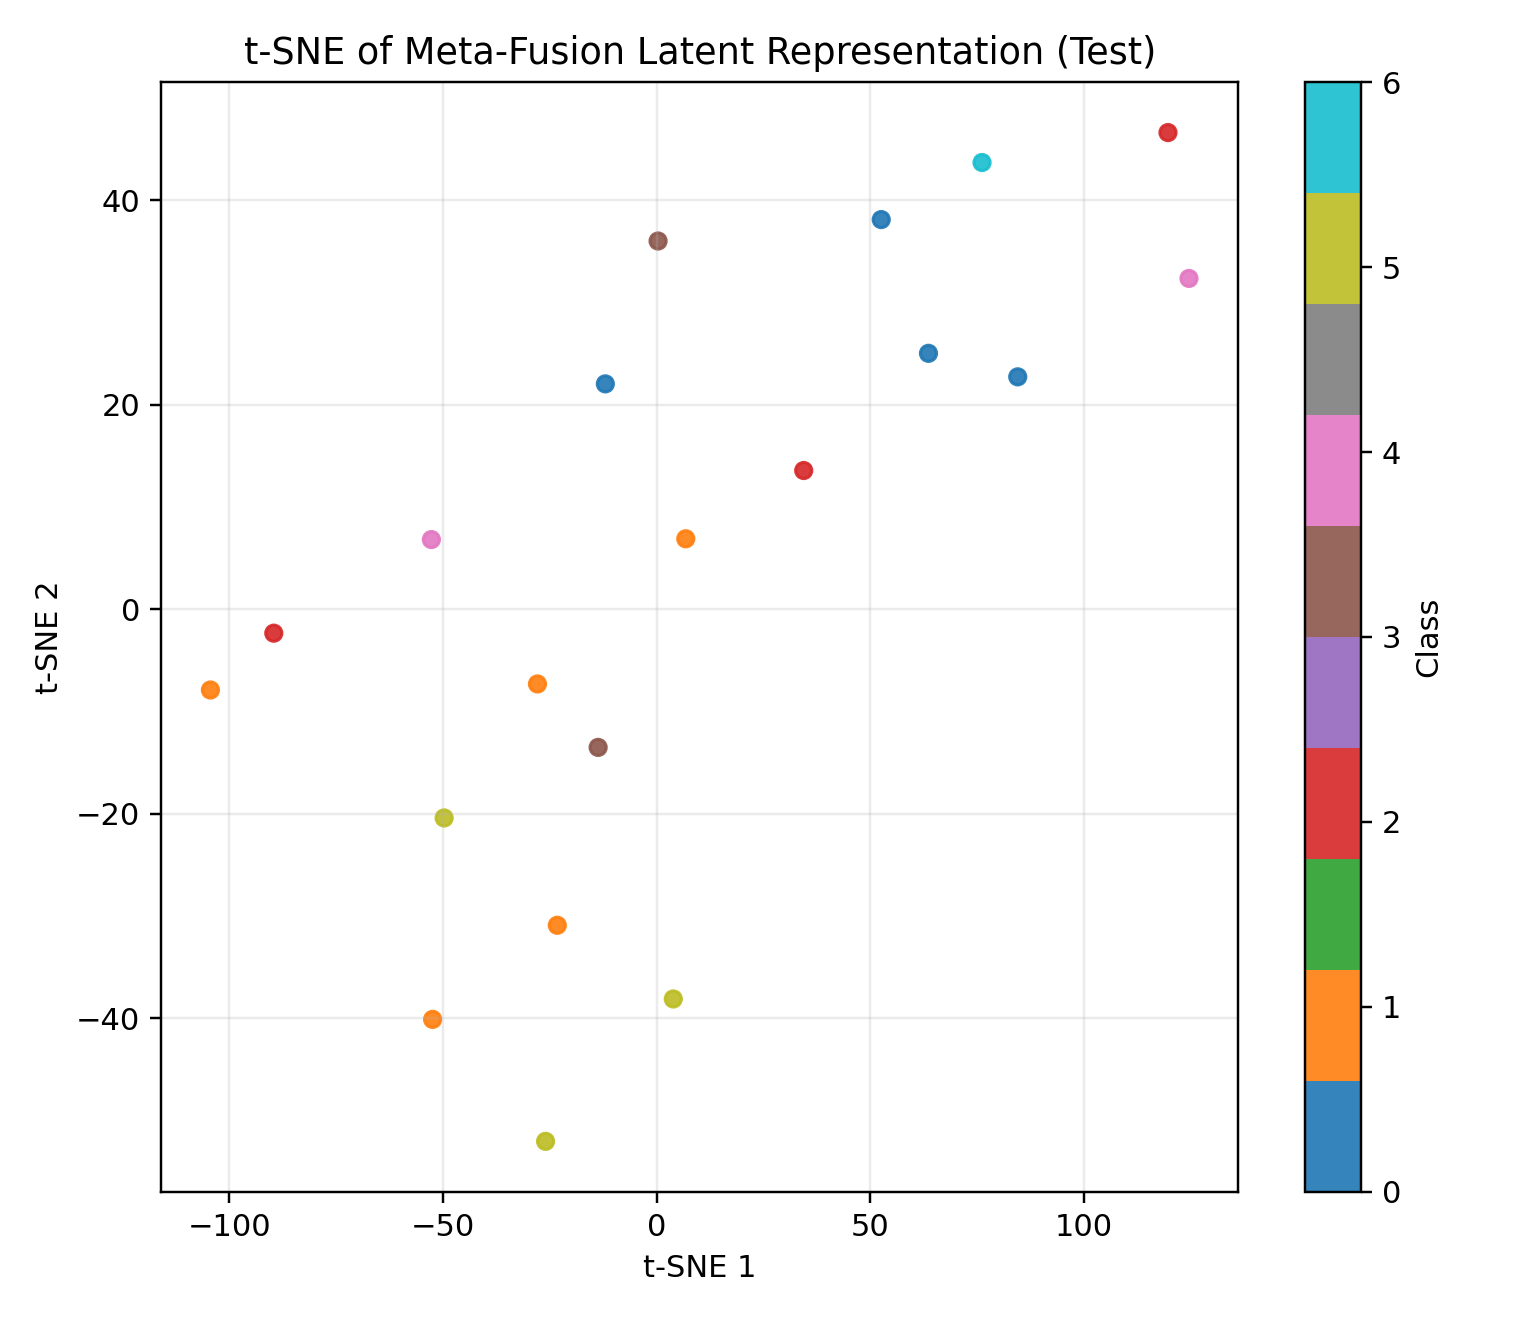
\includegraphics[width=\linewidth]{latent_tsne_meta_fusion.png}
	\caption{t-SNE projection}
	\label{fig:latent_tsne}
\end{subfigure}
\hfill
\begin{subfigure}{0.48\textwidth}
	\centering
	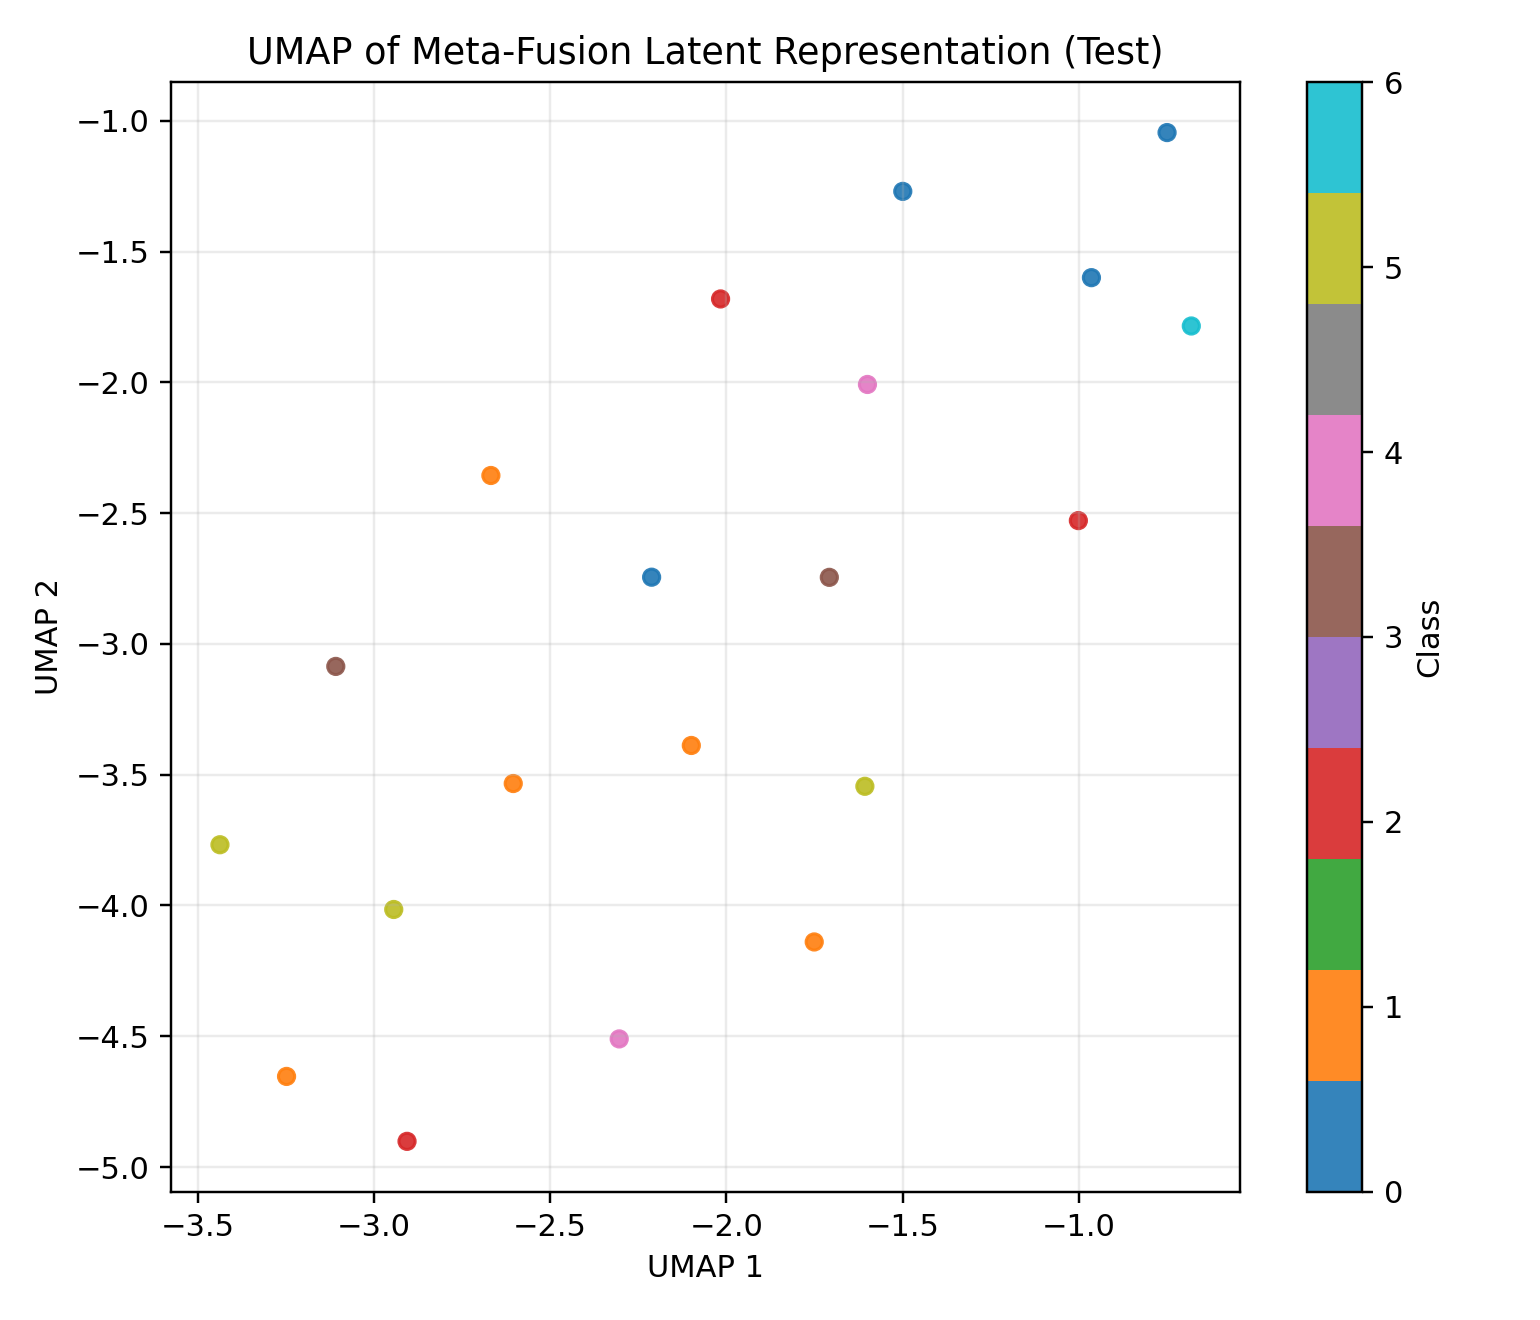
\includegraphics[width=\linewidth]{latent_umap_meta_fusion.png}
	\caption{UMAP projection}
	\label{fig:latent_umap}
\end{subfigure}
\caption{2D latent-space visualization of Meta-Fusion representations on the test set.}
\label{fig:latent_vis_combined}
\end{figure*}

As shown in Figures~\ref{fig:latent_tsne} and \ref{fig:latent_umap}, the fused latent space forms structured clusters with partial class overlap under the current low-data regime.

\section{Dimensionality and Downstream Comparison}

To quantify compression and utility, original concatenated features are compared with fused latent features.

\begin{table}[h]
\centering
\caption{Dimensionality Comparison}
\begin{tabular}{lc}
\toprule
Representation & Dimension \\
\midrule
Original concatenated & 84 \\
Meta-Fusion latent & 32 \\
Compression ratio (orig/latent) & 2.625 \\
\bottomrule
\end{tabular}
\end{table}

\begin{table}[h]
\centering
\caption{Classification: Original vs Latent}
\begin{tabular}{lccc}
\toprule
Representation & Accuracy & Macro-F1 & Macro-AUC \\
\midrule
Original concatenated & 0.35 & 0.3690 & 0.7604 \\
Meta-Fusion latent & 0.25 & 0.2023 & 0.5967 \\
\bottomrule
\end{tabular}
\end{table}

\begin{table}[h]
\centering
\caption{Clustering: Original vs Latent}
\begin{tabular}{lcc}
\toprule
Representation & ARI & NMI \\
\midrule
Original concatenated & 0.1695 & 0.5731 \\
Meta-Fusion latent & 0.0267 & 0.5063 \\
\bottomrule
\end{tabular}
\end{table}

\section{Cross-Dataset Generalization}

To improve generalization across datasets, several strategies are proposed:

\begin{itemize}
\item Domain-Adversarial Training
\item Progressive Multi-Dataset Training
\item Latent Feature Normalization
\end{itemize}

\section{Conclusion}

This work presented a Meta-Fusion Variational Autoencoder for multi-view speech emotion representation learning. The proposed architecture dynamically adapts fusion weights for multiple feature views and demonstrates robustness to corrupted modalities.

Experimental results show stable reconstruction learning and meaningful multi-class discrimination. In the current run, original concatenated features outperform latent features on classification and clustering, indicating that further latent regularization, larger-data training, and domain-adversarial objectives are required to fully realize the expected Meta-Fusion advantages. Future work will focus on larger datasets, distributed training, and stronger multimodal fusion mechanisms.

\begin{thebibliography}{00}

\bibitem{vae}
D. P. Kingma and M. Welling, ``Auto-Encoding Variational Bayes,'' ICLR, 2014.

\bibitem{domain}
Y. Ganin et al., ``Domain-Adversarial Training of Neural Networks,'' JMLR, 2016.

\bibitem{transformer}
A. Vaswani et al., ``Attention Is All You Need,'' NeurIPS, 2017.

\bibitem{ser}
S. Amiriparian et al., ``On the Impact of Acoustic Features in Speech Emotion Recognition,'' IEEE TASLP, 2017.

\end{thebibliography}

\end{document}
